% Author : Hakan OGUZ - Elektrik Elektronik Muhendisi
% Project: Rooftop 110 kWp grid-connected PV - layout and single-line design
% Date   : 2026-10-22
% License: MIT
\documentclass[11pt,a4paper]{article}
\usepackage[T1]{fontenc}
\usepackage[utf8]{inputenc}
\usepackage[english]{babel}
\usepackage{graphicx}
\usepackage{booktabs}
\usepackage{amsmath}
\usepackage{caption}
\usepackage{natbib}
\usepackage[margin=2.4cm]{geometry}
\graphicspath{{../sekiller/}}

\title{Electrical Design and Layout of a 110~kWp Rooftop\\ Grid-Connected Photovoltaic System}
\author{Hakan O\u{g}uz\\ \small Electrical and Electronics Engineer}
\date{October 2026}

\begin{document}
\maketitle

\begin{abstract}
This work documents the electrical design of a 110~kWp grid-connected photovoltaic (PV) array
placed on the flat roof of an industrial building. The design fixes the number of modules per
string from the low-temperature open-circuit voltage limit of the inverter, checks the maximum
power point tracking (MPPT) window at high cell temperature, and sizes the inter-row spacing from
the winter-solstice shading geometry at latitude 37$^\circ$. Twenty modules per string keep the
cold-string voltage at 1084~V, safely below the 1100~V inverter input ceiling, and ten strings
give a DC/AC ratio of 1.10. The results are expressed as two CAD sheets---a site layout and a
low-voltage single-line diagram---generated programmatically so that every dimension traces back
to the stated parameters.
\end{abstract}

\section{Introduction}
Rooftop PV plants in the 50--250~kWp range are a common way for industrial consumers to offset
daytime load. For a string inverter the first design decision is the string length, because the
array voltage must never exceed the inverter input rating, yet must stay inside the MPPT window
across the full operating temperature span~\citep{masters2013}. The open-circuit voltage of a
crystalline-silicon module rises as temperature falls, so the binding case is the coldest expected
cell temperature rather than standard test conditions~\citep{luque2011}. Alongside the voltage
chain, the layout must leave enough spacing between tilted rows to avoid mutual shading near solar
noon in winter. This paper carries a single 550~Wp module and a 100~kW inverter through these
checks and renders the outcome as dimensioned drawings. The requirements of IEC~62548 for PV array
design~\citep{iec62548} and IEC~60364-7-712 for PV installations~\citep{iec60364712} frame the
protection and earthing choices.

\section{Method}
\subsection{Components}
The array uses a 550~Wp monocrystalline module ($V_{oc}=49.5$~V, $V_{mp}=41.7$~V,
$I_{sc}=13.95$~A, $I_{mp}=13.19$~A, $\beta_{Voc}=-0.27~\%/^\circ$C, 2278$\times$1134~mm). The
inverter is a 100~kW unit with an MPPT window of 200--1000~V and a maximum DC input of 1100~V.
Table~\ref{tab:params} collects the figures used below.

\begin{table}[h]
\centering
\caption{Module and inverter parameters used in the design.}
\label{tab:params}
\begin{tabular}{llr}
\toprule
Item & Symbol & Value \\
\midrule
Module power (STC)        & $P_{mp}$        & 550 Wp \\
Open-circuit voltage       & $V_{oc}$        & 49.5 V \\
MPP voltage                & $V_{mp}$        & 41.7 V \\
$V_{oc}$ temp. coefficient & $\beta_{Voc}$   & $-0.27~\%/^\circ$C \\
Inverter max DC input      & $V_{dc,max}$    & 1100 V \\
Inverter MPPT window       & --              & 200--1000 V \\
\bottomrule
\end{tabular}
\end{table}

\subsection{String length from the cold-voltage limit}
With the coldest design cell temperature taken as $-10^\circ$C, the per-module open-circuit
voltage is
\begin{equation}
V_{oc}(T) = V_{oc,\mathrm{STC}}\,[1+\beta_{Voc}\,(T-25)]
          = 49.5\,[1+(-0.0027)(-10-25)] = 54.18~\text{V}.
\end{equation}
The number of modules per string follows from the inverter ceiling:
\begin{equation}
N_{max} = \frac{V_{dc,max}}{V_{oc}(-10^\circ\mathrm{C})} = \frac{1100}{54.18} = 20.3
\;\Rightarrow\; N = 20,
\end{equation}
giving a worst-case string voltage of $20\times54.18 = 1083.6$~V, below the 1100~V limit.

\subsection{MPPT window at high temperature}
Taking $\beta_{Vmp}\approx-0.34~\%/^\circ$C and a hot cell at $70^\circ$C,
\begin{equation}
V_{mp}(70^\circ\mathrm{C}) = 41.7\,[1+(-0.0034)(70-25)] = 35.3~\text{V},
\end{equation}
so the string works at $20\times35.3 = 706$~V when hot and $834$~V at STC---both inside the
200--1000~V window.

\subsection{Row spacing from shading geometry}
For a module tilt of $15^\circ$ the height and base projection of a landscape module (1.134~m
along the slope) are $h=1.134\sin15^\circ=0.293$~m and $b=1.134\cos15^\circ=1.095$~m. The winter
solstice noon solar altitude at latitude $37^\circ$ is $\alpha=90^\circ-37^\circ-23.45^\circ=
29.55^\circ$, so the shadow reaches $d=h/\tan\alpha=0.517$~m and the minimum pitch is
$p_{min}=b+d=1.61$~m. A pitch of 3.0~m was adopted to add a maintenance walkway.

\section{Results}
The array is organised as ten strings of twenty modules (200 modules, 110.0~kWp), which against
the 100~kW inverter gives a DC/AC ratio of 1.10. Figure~\ref{fig:layout} shows the generated site
plan: the ten colour-coded strings, the DC collection bus feeding the inverter and the AG
distribution panel, the perimeter earthing ring with corner electrodes, and the dimensioned roof
outline with the title block.

\begin{figure}[h]
\centering
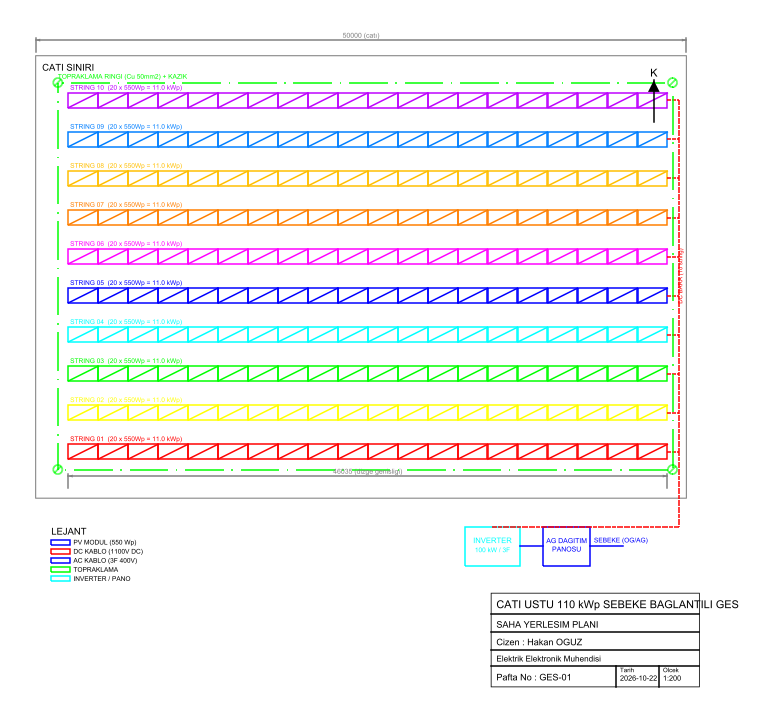
\includegraphics[width=0.96\textwidth]{saha-yerlesimi.png}
\caption{Generated site layout (sheet GES-01): ten strings, DC bus, inverter/panel, earthing ring.}
\label{fig:layout}
\end{figure}

Figure~\ref{fig:sld} gives the low-voltage single-line diagram. On the DC side each string carries
a 16~A gPV fuse, a Type~II DC surge arrester and an 1100~V DC disconnector; on the AC side the
inverter feeds a 160~A moulded-case breaker, a bidirectional meter and the AG distribution panel
before the grid. The 160~A breaker follows from the AC current
$I_{ac}=100\,000/(\sqrt{3}\cdot400\cdot0.98)\approx147$~A.

\begin{figure}[h]
\centering
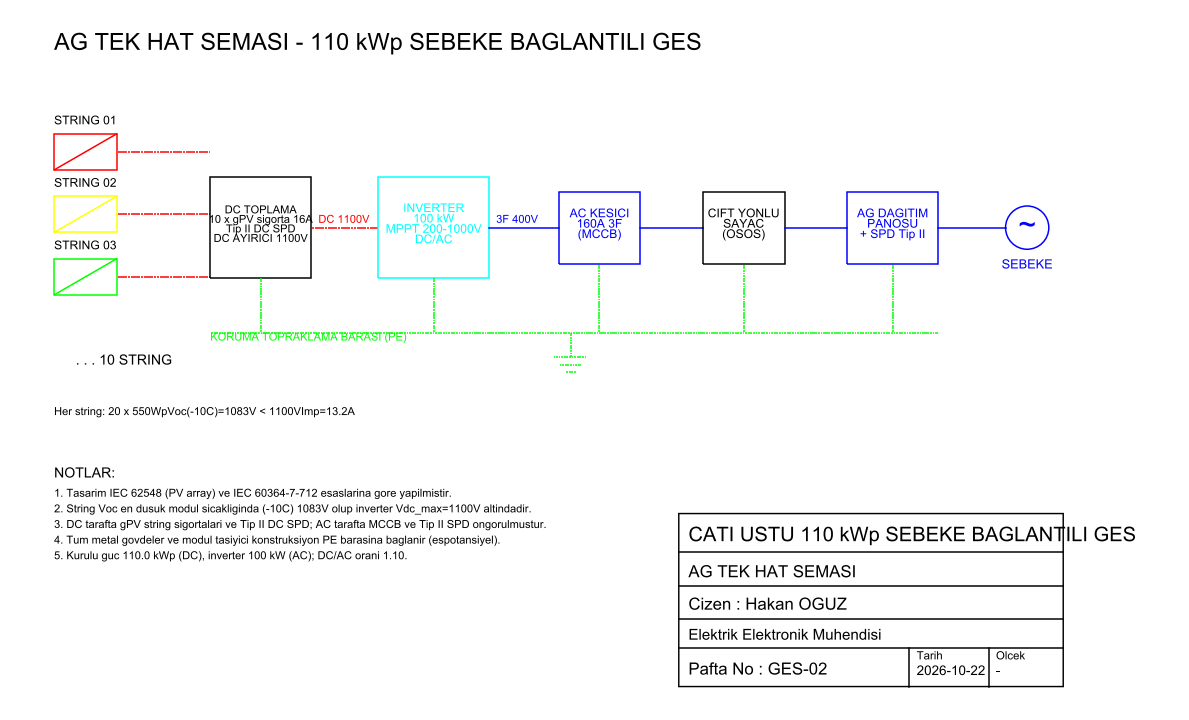
\includegraphics[width=0.96\textwidth]{tek-hat-semasi.png}
\caption{Generated single-line diagram (sheet GES-02) from string to grid connection.}
\label{fig:sld}
\end{figure}

Table~\ref{tab:results} summarises the sizing outcome. Every value in the drawings is derived from
the parameters in Table~\ref{tab:params}; changing a parameter in the generating script updates the
sheets consistently.

\begin{table}[h]
\centering
\caption{Design outcome.}
\label{tab:results}
\begin{tabular}{lr}
\toprule
Quantity & Value \\
\midrule
Modules per string              & 20 \\
Number of strings               & 10 \\
Installed DC power              & 110.0 kWp \\
Cold string voltage ($-10^\circ$C) & 1083.6 V \\
Hot string MPP voltage ($70^\circ$C) & 706 V \\
DC/AC ratio                     & 1.10 \\
AC current / main breaker       & 147 A / 160 A \\
Adopted row pitch               & 3.0 m \\
\bottomrule
\end{tabular}
\end{table}

\section{Conclusion}
A compact, parameter-driven procedure fixed the string length from the cold open-circuit voltage,
confirmed the MPPT window at high temperature, and set the row pitch from winter shading, yielding a
110~kWp array of ten twenty-module strings on a 100~kW inverter. Because the two CAD sheets are
produced from the same parameter set, the layout and the single-line diagram stay internally
consistent and are easy to revise for a different module or roof. The drawings are at preliminary
design level; a construction package would add structural, detailed cable-drop and utility
interconnection work.

\begin{thebibliography}{9}
\bibitem[International Electrotechnical Commission (2016)]{iec62548}
International Electrotechnical Commission. (2016). \textit{IEC 62548:2016 Photovoltaic (PV) arrays --
Design requirements}. IEC.

\bibitem[International Electrotechnical Commission (2017)]{iec60364712}
International Electrotechnical Commission. (2017). \textit{IEC 60364-7-712:2017 Low-voltage electrical
installations -- Part 7-712: Requirements for special installations or locations -- Solar photovoltaic
(PV) power supply systems}. IEC.

\bibitem[Luque \& Hegedus (2011)]{luque2011}
Luque, A., \& Hegedus, S. (Eds.). (2011). \textit{Handbook of photovoltaic science and engineering}
(2nd ed.). Wiley.

\bibitem[Masters (2013)]{masters2013}
Masters, G. M. (2013). \textit{Renewable and efficient electric power systems} (2nd ed.). Wiley.
\end{thebibliography}

\end{document}
